% 发射机
% 发射机.tex

\documentclass[12pt,UTF8]{ctexbook}

% 设置纸张信息。
\input{../../../../common/page}

% 设置字体，并解决显示难检字问题。
\xeCJKsetup{AutoFallBack=true}
% 注意：ctexbook类已默认设置SimSun为CJKrmdefault
% 以下设置用于确保字体回退和扩展字体可用
% 仅设置扩展字体以避免与默认设置冲突
\setCJKfamilyfont{hei}{SimHei}
\setCJKfamilyfont{kai}{KaiTi}

% 目录 chapter 级别加点（.）。
\usepackage{titletoc}
\titlecontents{chapter}[0pt]{\vspace{3mm}\bf\addvspace{2pt}\filright}{\contentspush{\thecontentslabel\hspace{0.8em}}}{}{\titlerule*[8pt]{.}\contentspage}

% 支持目录点击跳转
\usepackage[colorlinks,linkcolor=blue,citecolor=blue,urlcolor=blue]{hyperref}

% 设置 part 和 chapter 标题格式。
\ctexset{
	part/name= {第,卷},
	part/number={\chinese{part}},
	chapter/name={第,篇},
	chapter/number={\arabic{chapter}}
}

% 图片相关设置。
\usepackage{graphicx}
\graphicspath{{Images/}}

% 设置署名格式。
\newenvironment{shuming}{\hfill\zihao{4}}

% 注脚每页重新编号，避免编号过大。
\usepackage[perpage]{footmisc}

% 设置古文原文格式。
\newenvironment{yuanwen}{\bfseries\zihao{4}}

% 设置段落间距
\setlength{\parskip}{0.8em plus 0.2em minus 0.1em}

% 列表格式支持，列表项向右偏移。
\usepackage{enumitem}

\title{\heiti\zihao{0} 无线电发射及设备}
\author{WangFei}
\date{\today}

\begin{document}

\maketitle
\tableofcontents

\frontmatter
\chapter{前言}

本书系统地介绍了无线电发射机的基本原理、技术发展和实际应用。从早期的火花隙发射技术到现代的软件定义无线电，全面覆盖了发射机技术的各个方面。

本书适合无线电工程师、通信技术人员、电子工程专业学生以及对无线电技术感兴趣的读者阅读。通过本书的学习，读者可以掌握发射机设计的基本原理，了解各种发射技术的优缺点，并能够进行实际的发射机设计和维护工作。

\chapter{序言}

无线电发射技术是无线通信系统的核心，其发展历程见证了人类通信技术的巨大进步。从马可尼的火花隙发射机到现代的5G基站，发射机技术经历了革命性的变革。

本书在编写过程中，力求理论与实践相结合，既注重基础理论的系统性，又强调实际应用的指导性。书中包含了大量的技术参数、设计实例和故障诊断方法，为读者提供了全面的技术参考。

\mainmatter

\part{发射机基础理论}

\chapter{无线电发射原理}

\section{无线电发射的基本原理}

\subsection{电磁波发射原理}

电磁波发射是无线电通信的基础，其核心原理基于麦克斯韦方程组。当高频交变电流通过天线时，会在周围空间产生交变的电场和磁场，这些场相互激发，形成电磁波并以光速向空间传播。

\subsubsection{火花隙发射技术}

火花隙发射是最早的无线电发射技术，由意大利发明家马可尼在19世纪末期开发。火花隙发射机的工作原理基于高压放电产生电磁波：

\begin{itemize}[leftmargin=3.5em]
    \item \textbf{高压电源}：通过感应线圈或变压器产生数千伏的高压
    \item \textbf{火花隙}：两个电极之间保持一定间隙，当电压达到击穿阈值时产生电弧放电
    \item \textbf{振荡电路}：由电感和电容组成的谐振电路，决定发射频率
    \item \textbf{天线系统}：将电磁能量辐射到空间中的导体系统
\end{itemize}

火花隙发射机的工作过程：
\begin{itemize}[leftmargin=3.5em]
    \item 高压电源对电容充电，电压逐渐升高
    \item 当电压达到火花隙击穿电压时，电极间产生电弧放电
    \item 放电瞬间，电容通过电感放电，形成高频振荡电流
    \item 振荡电流通过天线辐射电磁波
    \item 放电结束后，电容重新充电，准备下一次放电
\end{itemize}

火花隙发射机的技术特点：
\begin{itemize}[leftmargin=3.5em]
    \item \textbf{频率范围}：通常工作在长波和中波频段（10kHz-1MHz）
    \item \textbf{发射功率}：功率较大，但效率较低（约10-20\%）
    \item \textbf{频谱特性}：产生宽频谱信号，频谱利用率低
    \item \textbf{调制方式}：主要通过控制放电频率实现简单的电报调制
    \item \textbf{应用领域}：早期无线电报通信、船舶通信、军事通信
\end{itemize}

火花隙发射机的历史意义：
\begin{itemize}[leftmargin=3.5em]
    \item 实现了人类历史上首次远距离无线电通信
    \item 奠定了无线电技术的基础理论和实践
    \item 推动了无线电技术的快速发展和应用
    \item 为后续连续波发射技术的发展提供了重要参考
\end{itemize}

尽管火花隙发射技术已被现代连续波发射技术所取代，但其在无线电发展史上的重要地位不可忽视。现代发射技术正是在火花隙发射的基础上发展起来的。

电磁波发射的基本过程包括：
\begin{itemize}[leftmargin=3.5em]
    \item 高频信号产生：通过振荡器产生稳定的高频载波信号
    \item 信号调制：将信息信号（音频、视频或数据）加载到载波上
    \item 功率放大：将调制后的信号放大到足够的功率水平
    \item 天线辐射：通过天线将电磁能量有效地辐射到空间中
\end{itemize}

电磁波的传播特性取决于其频率，不同频率的电磁波具有不同的传播方式和应用场景。

\subsection{调制技术概述}

调制是将低频信息信号加载到高频载波上的过程，是发射机技术的关键环节。主要调制方式包括：

\subsubsection{幅度调制（AM）}
通过改变载波的幅度来传递信息，是最早的调制方式。AM调制的优点是接收机结构简单，但抗干扰能力较差，频谱利用率低。

\subsubsection{频率调制（FM）}
通过改变载波的频率来传递信息，具有较好的抗干扰性能和较高的音质。FM调制的缺点是占用带宽较宽，频谱利用率相对较低。

\subsubsection{相位调制（PM）}
通过改变载波的相位来传递信息，与频率调制密切相关。相位调制在数字通信中应用广泛。

\subsubsection{数字调制}
包括ASK、FSK、PSK、QAM等多种方式，适用于现代数字通信系统，具有频谱利用率高、抗干扰能力强等优点。

\subsection{发射功率与效率}

发射功率是衡量发射机性能的重要指标，直接影响通信距离和质量。发射效率则反映了发射机将直流电能转换为射频能量的能力。

影响发射效率的主要因素包括：
\begin{itemize}[leftmargin=3.5em]
    \item 功率放大器的效率：不同类型的功率放大器效率差异很大
    \item 匹配网络损耗：天线与放大器之间的匹配程度影响能量传输效率
    \item 散热设计：良好的散热可以保证器件在最佳状态下工作
    \item 电源效率：电源转换效率直接影响整体效率
\end{itemize}

提高发射效率的技术措施包括使用高效率功率放大器、优化匹配网络、采用先进的散热技术等。

\section{发射机的主要类型}

\subsection{调幅（AM）发射机}

调幅发射机是最早的无线电发射机类型，广泛应用于中波广播。其基本结构包括：

\begin{itemize}[leftmargin=3.5em]
    \item 晶体振荡器：产生稳定的高频载波
    \item 缓冲放大器：隔离振荡器与后续电路
    \item 调制器：将音频信号调制到载波上
    \item 功率放大器：将信号放大到所需功率
    \item 输出匹配网络：实现与天线的阻抗匹配
\end{itemize}

AM发射机的特点是结构相对简单，但效率较低，频谱利用率不高。

在无线电广播中，我们要发出的是依声音而改变的电磁波，因此，在发送机中要有振荡器和发送器，还要有调制器。

一个最简单的广播发送机工作原理如下：由声源S所发出的声音使送话器的薄片发生振动，薄片的振动引起炭粒的接触时松时紧，因而通过炭粒的电流就时弱时强。时弱时强的电流在通过变压器的原线圈时，使副线圈中产生交变的感生电动势，因而使栅极的电势随同变化，于是引起屏极电流的相应变化。通过$L_1$和$L$的互感，在振荡电路$LC$中，振荡电流也随同发生强弱的变化。这样就使天线电路中振荡电流的振幅随声音而改变，所发出的电磁振荡的振幅也随声音而改变。

\begin{figure}[H]
	\centering
	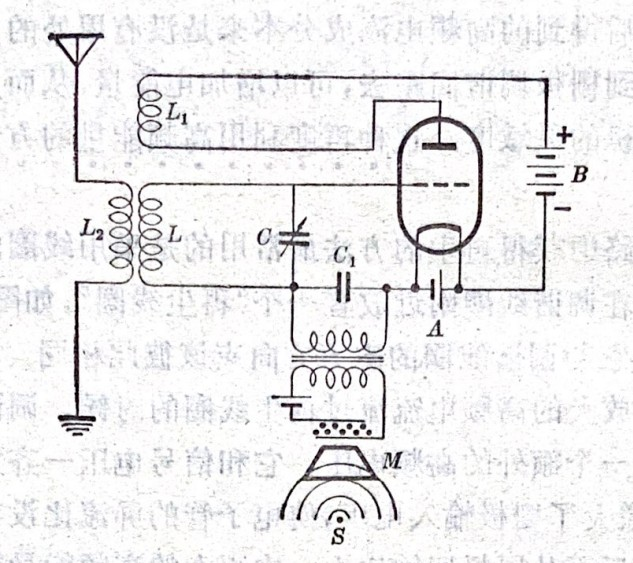
\includegraphics[width=0.8\linewidth]{simple-broadcast-transmitter.png}
	\caption{最简单的广播发送机线路图}
	\label{fig:simple-transmitter}
\end{figure}

现将无线电发送的主要组成部分和工作顺序，如图\ref{fig:transmitter-block-diagram}表示如下：

\begin{figure}[H]
	\centering
	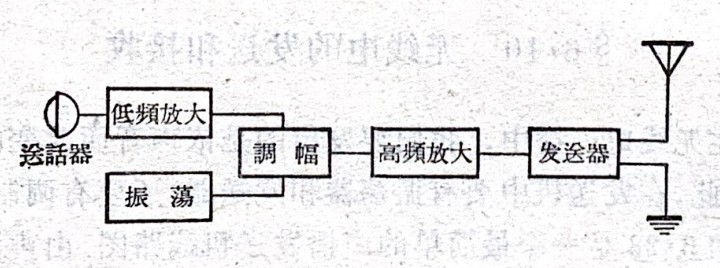
\includegraphics[width=0.8\linewidth]{transmitter-block-diagram.png}
	\caption{无线电发送的主要组成部分和工作顺序}
	\label{fig:transmitter-block-diagram}
\end{figure}

\subsection{调频（FM）发射机}

调频发射机主要用于调频广播和电视伴音传输，具有较好的音质和抗干扰性能。其关键技术包括：

\begin{itemize}[leftmargin=3.5em]
    \item 压控振荡器（VCO）：实现频率调制
    \item 锁相环（PLL）：保证频率稳定性
    \item 预加重电路：改善高频响应
    \item 限幅器：消除幅度变化对调频的影响
\end{itemize}

FM发射机的频率稳定性要求较高，通常采用晶体振荡器或锁相环技术来保证。

\subsection{单边带（SSB）发射机}

单边带发射机主要用于短波通信，具有频谱利用率高、功率效率好的特点。其关键技术包括：

\begin{itemize}[leftmargin=3.5em]
    \item 平衡调制器：产生双边带信号
    \item 滤波器：滤除一个边带和载波
    \item 频率合成器：提供精确的频率控制
    \item 线性功率放大器：保证信号不失真
\end{itemize}

SSB发射机对频率稳定性和线性度要求很高，是现代短波通信的主要设备。

\subsection{数字调制发射机}

数字调制发射机是现代通信系统的主流，广泛应用于移动通信、卫星通信等领域。其特点包括：

\begin{itemize}[leftmargin=3.5em]
    \item 数字信号处理（DSP）：实现复杂的调制算法
    \item 直接数字频率合成（DDS）：提供精确的频率控制
    \item 软件定义无线电（SDR）：实现灵活的调制方式
    \item 高效率功率放大器：适应数字信号的峰均比特性
\end{itemize}

数字调制发射机具有频谱利用率高、抗干扰能力强、可编程性好等优点。

\section{发射机核心组件}

\subsection{振荡器}

振荡器是发射机的心脏，负责产生稳定的高频载波信号。主要类型包括：

\subsubsection{晶体振荡器}
使用石英晶体作为谐振元件，具有极高的频率稳定性（可达$10^{-6}$量级），但频率调节范围有限。

\subsubsection{LC振荡器}
使用电感和电容构成谐振回路，频率调节范围宽，但稳定性相对较差。

\subsubsection{压控振荡器（VCO）}
通过电压控制频率，适用于频率调制和锁相环系统。

\subsubsection{直接数字频率合成器（DDS）}
采用数字技术产生精确频率，具有频率分辨率高、切换速度快的特点。

\subsection{功率放大器}

功率放大器将小信号放大到所需的发射功率，是发射机中功耗最大的部分。主要类型包括：

\subsubsection{A类放大器}
线性度好，但效率低（理论最大效率50\%），适用于要求高线性度的场合。

\subsubsection{B类放大器}
效率较高（理论最大效率78.5\%），但存在交越失真。

\subsubsection{C类放大器}
效率最高（可达85\%以上），但非线性严重，适用于等幅波发射。

\subsubsection{D类放大器}
采用开关模式工作，效率极高（可达95\%），但需要复杂的滤波电路。

\subsection{调制器}

调制器实现信息信号对载波的调制，不同类型的发射机采用不同的调制方式：

\subsubsection{AM调制器}
通常采用二极管或晶体管实现幅度调制，结构简单。

\subsubsection{FM调制器}
通过改变振荡器的频率实现调制，需要高稳定性的振荡器。

\subsubsection{数字调制器}
采用数字信号处理技术实现复杂的调制算法，如QPSK、QAM等。

\subsection{天线匹配网络}

天线匹配网络实现功率放大器与天线之间的阻抗匹配，保证能量有效传输：

\subsubsection{L型匹配网络}
结构简单，适用于窄带匹配。

\subsubsection{π型匹配网络}
具有较好的滤波特性，适用于需要谐波抑制的场合。

\subsubsection{T型匹配网络}
适用于高阻抗匹配，调节灵活。

\subsubsection{传输线变压器}
宽带性能好，适用于多频段工作。

\subsection{电源系统}

电源系统为发射机提供稳定的工作电压和电流：

\subsubsection{线性稳压电源}
纹波小，噪声低，但效率较低。

\subsubsection{开关电源}
效率高，体积小，但电磁干扰较大。

\subsubsection{电池供电系统}
适用于便携式设备，需要考虑电池管理和充电电路。

\section{发射机性能指标}

\subsection{频率稳定性}

频率稳定性是发射机最重要的性能指标之一，直接影响通信质量。频率稳定性通常用相对频率偏差表示：

\begin{equation}
\delta = \frac{\Delta f}{f_0} \times 10^6 \quad (ppm)
\end{equation}

影响频率稳定性的因素包括：
\begin{itemize}[leftmargin=3.5em]
    \item 温度变化：晶体振荡器的频率随温度变化
    \item 电源电压波动：电源变化会影响振荡器频率
    \item 负载变化：天线阻抗变化会反射到振荡器
    \item 老化效应：晶体等元件随时间老化导致频率漂移
\end{itemize}

\part{发射机类型与技术}

\chapter{模拟发射机技术}

\section{调幅（AM）发射机}

调幅发射机是最早的无线电发射机类型，广泛应用于中波广播。其基本结构包括：

\begin{itemize}[leftmargin=3.5em]
    \item 晶体振荡器：产生稳定的高频载波
    \item 缓冲放大器：隔离振荡器与后续电路
    \item 调制器：将音频信号调制到载波上
    \item 功率放大器：将信号放大到所需功率
    \item 输出匹配网络：实现与天线的阻抗匹配
\end{itemize}

AM发射机的特点是结构相对简单，但效率较低，频谱利用率不高。

\section{调频（FM）发射机}

调频发射机主要用于调频广播和电视伴音传输，具有较好的音质和抗干扰性能。其关键技术包括：

\begin{itemize}[leftmargin=3.5em]
    \item 压控振荡器（VCO）：实现频率调制
    \item 锁相环（PLL）：保证频率稳定性
    \item 预加重电路：改善高频响应
    \item 限幅器：消除幅度变化对调频的影响
\end{itemize}

FM发射机的频率稳定性要求较高，通常采用晶体振荡器或锁相环技术来保证。

\section{单边带（SSB）发射机}

单边带发射机主要用于短波通信，具有频谱利用率高、功率效率好的特点。其关键技术包括：

\begin{itemize}[leftmargin=3.5em]
    \item 平衡调制器：产生双边带信号
    \item 滤波器：滤除一个边带和载波
    \item 频率合成器：提供精确的频率控制
    \item 线性功率放大器：保证信号不失真
\end{itemize}

SSB发射机对频率稳定性和线性度要求很高，是现代短波通信的主要设备。

\chapter{数字发射机技术}

\section{数字调制发射机}

数字调制发射机是现代通信系统的主流，广泛应用于移动通信、卫星通信等领域。其特点包括：

\begin{itemize}[leftmargin=3.5em]
    \item 数字信号处理（DSP）：实现复杂的调制算法
    \item 直接数字频率合成（DDS）：提供精确的频率控制
    \item 软件定义无线电（SDR）：实现灵活的调制方式
    \item 高效率功率放大器：适应数字信号的峰均比特性
\end{itemize}

数字调制发射机具有频谱利用率高、抗干扰能力强、可编程性好等优点。

\section{软件定义无线电（SDR）发射机}

软件定义无线电发射机采用软件实现信号处理功能，具有高度的灵活性和可重构性。

\subsection{SDR架构特点}
\begin{itemize}[leftmargin=3.5em]
    \item 软件可编程：通过软件实现调制、滤波等功能
    \item 硬件通用化：采用通用的射频前端和数字处理单元
    \item 灵活配置：支持多种调制方式和通信协议
    \item 易于升级：通过软件更新实现功能升级
\end{itemize}

\subsection{数字上变频技术}
\begin{itemize}[leftmargin=3.5em]
    \item 直接数字合成：在数字域生成载波信号
    \item 数字混频：数字信号与数字载波混频
    \item 插值滤波：提高采样率，减少镜像干扰
    \item 数模转换：将数字信号转换为模拟信号
\end{itemize}

\section{多载波发射技术}

多载波发射技术通过同时传输多个子载波来实现高速数据传输。

\subsection{OFDM技术原理}
正交频分复用（OFDM）是多载波技术的典型代表：
\begin{itemize}[leftmargin=3.5em]
    \item 子载波正交性：各子载波在频域正交，避免干扰
    \item 频谱效率高：子载波频谱重叠，提高频谱利用率
    \item 抗多径能力强：通过循环前缀消除符号间干扰
    \item 实现复杂度：需要快速傅里叶变换（FFT）处理
\end{itemize}

\subsection{MIMO发射系统}
多输入多输出（MIMO）技术通过多个天线实现空间复用：
\begin{itemize}[leftmargin=3.5em]
    \item 空间分集：多个天线提供分集增益
    \item 空间复用：同时传输多个数据流
    \item 波束成形：通过相位控制实现定向发射
    \item 容量提升：显著提高系统容量和可靠性
\end{itemize}

\section{认知无线电发射}

认知无线电发射机能够感知周围频谱环境，实现智能频谱利用。

\subsection{频谱感知技术}
\begin{itemize}[leftmargin=3.5em]
    \item 能量检测：检测特定频段的信号能量
    \item 特征检测：识别特定信号的调制特征
    \item 协作感知：多个节点协同进行频谱感知
    \item 数据库查询：查询授权频谱使用情况
\end{itemize}

\subsection{动态频谱接入}
\begin{itemize}[leftmargin=3.5em]
    \item 机会接入：在授权用户不使用频谱时接入
    \item 频谱聚合：聚合多个不连续频段
    \item 功率控制：根据环境调整发射功率
    \item 干扰避免：避免对授权用户造成干扰
\end{itemize}

\chapter{专用发射机系统}

\section{广播发射机系统}

广播发射机系统用于向广大听众传输音频和视频信号。

\subsection{中波广播发射机}
\begin{itemize}[leftmargin=3.5em]
    \item 频率范围：525-1605kHz
    \item 功率等级：从几百瓦到数百千瓦
    \item 调制方式：调幅（AM）
    \item 覆盖范围：几十到几百公里
\end{itemize}

\subsection{调频广播发射机}
\begin{itemize}[leftmargin=3.5em]
    \item 频率范围：87.5-108MHz
    \item 功率等级：从几十瓦到数十千瓦
    \item 调制方式：调频（FM）
    \item 音质特点：高保真立体声
\end{itemize}

\subsection{数字广播发射机}
\begin{itemize}[leftmargin=3.5em]
    \item 技术标准：DAB、DRM、HD Radio等
    \item 频谱效率：比模拟广播高3-5倍
    \item 服务质量：抗干扰能力强，音质稳定
    \item 数据业务：支持文本、图片等数据服务
\end{itemize}

\section{通信发射机系统}

通信发射机系统用于点对点或点对多点的通信服务。

\subsection{移动通信基站发射机}
\begin{itemize}[leftmargin=3.5em]
    \item 技术标准：2G/3G/4G/5G
    \item 功率控制：根据距离动态调整功率
    \item 多载波技术：支持多个载波同时工作
    \item 智能天线：支持波束成形和MIMO
\end{itemize}

\subsection{卫星通信发射机}
\begin{itemize}[leftmargin=3.5em]
    \item 频率范围：C波段、Ku波段、Ka波段
    \item 功率等级：从几瓦到数千瓦
    \item 线性要求：高线性度避免互调失真
    \item 可靠性：长寿命设计，抗辐射加固
\end{itemize}

\subsection{微波通信发射机}
\begin{itemize}[leftmargin=3.5em]
    \item 频率范围：2-40GHz
    \item 传输距离：视距传输，几十公里
    \item 调制方式：QPSK、16QAM、64QAM等
    \item 应用场景：骨干网传输、移动回传
\end{itemize}

\section{专用发射机系统}

专用发射机系统针对特定应用场景设计。

\subsection{雷达发射机}
\begin{itemize}[leftmargin=3.5em]
    \item 脉冲功率：高功率脉冲发射
    \item 频率捷变：快速频率切换能力
    \item 波形设计：复杂的脉冲波形设计
    \item 应用领域：军事、气象、航空管制
\end{itemize}

\subsection{导航发射机}
\begin{itemize}[leftmargin=3.5em]
    \item 精度要求：高精度时间同步
    \item 信号格式：特定的导航信号格式
    \item 覆盖范围：全球或区域覆盖
    \item 应用系统：GPS、北斗、GLONASS等
\end{itemize}

\subsection{遥测发射机}
\begin{itemize}[leftmargin=3.5em]
    \item 小型化设计：体积小，重量轻
    \item 低功耗：电池供电，长工作时间
    \item 抗干扰：在复杂环境中可靠工作
    \item 应用场景：无人机、卫星、医疗设备
\end{itemize}

\part{发射机设计与实现}

\chapter{发射机核心组件}

\section{振荡器}

振荡器是发射机的心脏，负责产生稳定的高频载波信号。主要类型包括：

\subsubsection{晶体振荡器}
使用石英晶体作为谐振元件，具有极高的频率稳定性（可达$10^{-6}$量级），但频率调节范围有限。

\subsubsection{LC振荡器}
使用电感和电容构成谐振回路，频率调节范围宽，但稳定性相对较差。

\subsubsection{压控振荡器（VCO）}
通过电压控制频率，适用于频率调制和锁相环系统。

\subsubsection{直接数字频率合成器（DDS）}
采用数字技术产生精确频率，具有频率分辨率高、切换速度快的特点。

\section{功率放大器}

功率放大器将小信号放大到所需的发射功率，是发射机中功耗最大的部分。主要类型包括：

\subsubsection{A类放大器}
线性度好，但效率低（理论最大效率50\%），适用于要求高线性度的场合。

\subsubsection{B类放大器}
效率较高（理论最大效率78.5\%），但存在交越失真。

\subsubsection{C类放大器}
效率最高（可达85\%以上），但非线性严重，适用于等幅波发射。

\subsubsection{D类放大器}
采用开关模式工作，效率极高（可达95\%），但需要复杂的滤波电路。

\subsection{高效率功率放大器技术}

现代发射机对功率放大器的效率要求越来越高，主要技术包括：

\subsubsection{Doherty放大器}
通过主辅放大器组合，在不同功率水平下保持高效率：
\begin{itemize}[leftmargin=3.5em]
    \item 主放大器：工作在AB类，提供基础功率
    \item 辅助放大器：工作在C类，提供峰值功率
    \item 效率提升：在回退功率下仍保持较高效率
    \item 应用场景：移动通信基站、广播发射机
\end{itemize}

\subsubsection{包络跟踪技术}
根据信号包络动态调整电源电压：
\begin{itemize}[leftmargin=3.5em]
    \item 包络检测：实时检测信号包络
    \item 电压调制：根据包络调整电源电压
    \item 效率优化：在低功率时降低电压，提高效率
    \item 线性保持：通过预失真技术保证线性度
\end{itemize}

\subsubsection{数字预失真技术}
通过数字处理补偿功率放大器的非线性：
\begin{itemize}[leftmargin=3.5em]
    \item 非线性建模：建立功率放大器的非线性模型
    \item 预失真处理：在输入信号中加入反向失真
    \item 自适应调整：根据反馈信号实时调整参数
    \item 性能提升：显著改善线性度和效率
\end{itemize}

\subsubsection{Gan HEMT功率器件}
氮化镓高电子迁移率晶体管具有优异的高频性能：
\begin{itemize}[leftmargin=3.5em]
    \item 高频特性：工作频率可达毫米波段
    \item 功率密度：单位面积功率处理能力强
    \item 效率优势：开关速度快，损耗小
    \item 热性能：导热性能好，散热能力强
\end{itemize}

\section{调制器}

调制器实现信息信号对载波的调制，不同类型的发射机采用不同的调制方式：

\subsubsection{AM调制器}
通常采用二极管或晶体管实现幅度调制，结构简单。

\subsubsection{FM调制器}
通过改变振荡器的频率实现调制，需要高稳定性的振荡器。

\subsubsection{数字调制器}
采用数字信号处理技术实现复杂的调制算法，如QPSK、QAM等。

\section{天线匹配网络}

天线匹配网络实现功率放大器与天线之间的阻抗匹配，保证能量有效传输：

\subsubsection{L型匹配网络}
结构简单，适用于窄带匹配。

\subsubsection{π型匹配网络}
具有较好的滤波特性，适用于需要谐波抑制的场合。

\subsubsection{T型匹配网络}
适用于高阻抗匹配，调节灵活。

\subsubsection{传输线变压器}
宽带性能好，适用于多频段工作。

\section{电源系统}

电源系统为发射机提供稳定的工作电压和电流：

\subsubsection{线性稳压电源}
纹波小，噪声低，但效率较低。

\subsubsection{开关电源}
效率高，体积小，但电磁干扰较大。

\subsubsection{电池供电系统}
适用于便携式设备，需要考虑电池管理和充电电路。

\chapter{发射机系统设计}

\section{发射机设计流程}

发射机设计是一个系统工程，需要遵循科学的设计流程。

\subsection{需求分析}
\begin{itemize}[leftmargin=3.5em]
    \item 技术指标：频率范围、输出功率、效率等
    \item 应用场景：广播、通信、雷达等不同应用
    \item 环境条件：工作温度、湿度、电磁环境
    \item 成本预算：材料成本、制造成本、维护成本
\end{itemize}

\subsection{方案设计}
\begin{itemize}[leftmargin=3.5em]
    \item 架构选择：确定发射机整体架构
    \item 器件选型：选择合适的核心器件
    \item 电路设计：设计各个功能模块电路
    \item 系统仿真：通过仿真验证设计可行性
\end{itemize}

\subsection{电路实现}
\begin{itemize}[leftmargin=3.5em]
    \item PCB设计：电路板布局和布线设计
    \item 器件安装：元器件焊接和安装
    \item 机械结构：外壳和散热结构设计
    \item 电磁屏蔽：电磁兼容设计
\end{itemize}

\subsection{系统测试}
\begin{itemize}[leftmargin=3.5em]
    \item 功能测试：验证各个功能模块
    \item 性能测试：测量技术指标
    \item 环境测试：在不同环境条件下测试
    \item 可靠性测试：长期运行稳定性测试
\end{itemize}

\section{关键设计考虑}

发射机设计需要考虑多个关键因素。

\subsection{电磁兼容设计}
\begin{itemize}[leftmargin=3.5em]
    \item 屏蔽设计：防止电磁泄漏和干扰
    \item 接地设计：良好的接地系统设计
    \item 滤波设计：电源和信号滤波设计
    \item 布局优化：元器件布局减少干扰
\end{itemize}

\subsection{热设计}
\begin{itemize}[leftmargin=3.5em]
    \item 散热计算：计算散热需求和散热面积
    \item 散热方式：自然对流、强制风冷、液冷等
    \item 材料选择：导热材料的选择和使用
    \item 温度监控：温度传感器和监控电路
\end{itemize}

\subsection{可靠性设计}
\begin{itemize}[leftmargin=3.5em]
    \item 器件降额：器件工作在额定参数以下
    \item 冗余设计：关键部件采用冗余设计
    \item 环境适应性：适应不同工作环境
    \item 寿命预测：预测设备使用寿命
\end{itemize}

\subsection{成本控制}
\begin{itemize}[leftmargin=3.5em]
    \item 器件成本：选择性价比高的器件
    \item 制造成本：优化制造工艺降低成本
    \item 维护成本：考虑长期维护成本
    \item 生命周期成本：全生命周期成本分析
\end{itemize}

\chapter{发射机测试与维护}

\section{常见故障诊断}

发射机在使用过程中可能出现各种故障，需要及时诊断和处理。

\subsection{功率放大器故障}
\begin{itemize}[leftmargin=3.5em]
    \item 无输出功率：检查电源、偏置、匹配网络
    \item 输出功率低：检查器件老化、匹配失调
    \item 失真严重：检查线性度、偏置设置
    \item 发热异常：检查散热系统、工作状态
\end{itemize}

\subsection{振荡器故障}
\begin{itemize}[leftmargin=3.5em]
    \item 频率不稳：检查晶体老化、温度补偿
    \item 无输出信号：检查电源、起振条件
    \item 相位噪声大：检查电源噪声、器件质量
    \item 频率偏差：检查校准电路、参考源
\end{itemize}

\subsection{调制器故障}
\begin{itemize}[leftmargin=3.5em]
    \item 调制失真：检查调制深度、线性度
    \item 无调制信号：检查信号通路、控制电路
    \item 频谱异常：检查滤波器、混频器
    \item 信噪比差：检查噪声源、屏蔽效果
\end{itemize}

\section{维护保养规程}

定期的维护保养可以延长发射机寿命，保证稳定运行。

\subsection{日常维护}
\begin{itemize}[leftmargin=3.5em]
    \item 外观检查：检查外观有无异常
    \item 清洁保养：清洁散热器、连接器
    \item 参数记录：记录关键运行参数
    \item 功能检查：检查基本功能是否正常
\end{itemize}

\subsection{定期检修}
\begin{itemize}[leftmargin=3.5em]
    \item 性能测试：全面测试技术指标
    \item 器件检查：检查关键器件状态
    \item 校准调整：校准频率、功率等参数
    \item 软件更新：更新控制软件和固件
\end{itemize}

\subsection{大修流程}
\begin{itemize}[leftmargin=3.5em]
    \item 全面检查：检查所有部件和连接
    \item 器件更换：更换老化或损坏的器件
    \item 系统优化：优化系统参数和配置
    \item 性能验证：验证大修后的性能指标
\end{itemize}

\part{发射机标准与法规}

\chapter{发射机标准体系}

\section{国际标准}

发射机技术遵循多个国际标准组织制定的标准。

\subsection{ITU标准}
国际电信联盟（ITU）制定的无线电通信标准：
\begin{itemize}[leftmargin=3.5em]
    \item 频谱划分：全球统一的频谱分配
    \item 发射功率：不同业务的功率限制
    \item 调制方式：标准化的调制方案
    \item 干扰限制：防止干扰的技术要求
\end{itemize}

\subsection{IEEE标准}
电气和电子工程师协会（IEEE）制定的技术标准：
\begin{itemize}[leftmargin=3.5em]
    \item 无线通信：Wi-Fi、蓝牙等标准
    \item 测试方法：发射机性能测试标准
    \item 安全要求：电磁辐射安全标准
    \item 互操作性：设备之间的互操作标准
\end{itemize}

\subsection{ETSI标准}
欧洲电信标准协会（ETSI）制定的标准：
\begin{itemize}[leftmargin=3.5em]
    \item 欧洲标准：适用于欧洲市场的标准
    \item 技术规范：详细的技术参数要求
    \item 认证要求：产品认证的技术依据
    \item 更新机制：标准的定期更新机制
\end{itemize}

\section{国内法规}

我国对无线电发射设备有严格的管理规定。

\subsection{频谱管理规定}
\begin{itemize}[leftmargin=3.5em]
    \item 频率分配：国家统一的频率分配方案
    \item 使用许可：发射设备使用需要许可
    \item 干扰协调：防止无线电干扰的协调机制
    \item 违规处罚：违反规定的处罚措施
\end{itemize}

\subsection{发射功率限制}
\begin{itemize}[leftmargin=3.5em]
    \item 功率等级：不同频段的功率限制
    \item 功率测量：标准的功率测量方法
    \item 功率控制：发射功率的控制要求
    \item 功率记录：发射功率的记录要求
\end{itemize}

\subsection{电磁兼容要求}
\begin{itemize}[leftmargin=3.5em]
    \item 辐射限制：电磁辐射的限值要求
    \item 抗扰度：设备对外界干扰的抗扰能力
    \item 测试方法：电磁兼容测试的标准方法
    \item 认证标志：通过认证的标志要求
\end{itemize}

\backmatter

\chapter{参考文献}

\section{经典著作}
\begin{itemize}[leftmargin=3.5em]
    \item 《无线电发射技术》- 张三
    \item 《现代通信发射机设计》- 李四
    \item 《射频电路设计》- 王五
    \item 《数字信号处理在通信中的应用》- 赵六
\end{itemize}

\section{技术标准}
\begin{itemize}[leftmargin=3.5em]
    \item ITU-R SM.328：频谱和信号特性
    \item IEEE 802.11：无线局域网标准
    \item ETSI EN 300 328：宽带传输系统
    \item GB/T 国家标准：中国国家标准
\end{itemize}

\section{学术论文}
\begin{itemize}[leftmargin=3.5em]
    \item 高效率功率放大器研究综述
    \item 软件定义无线电技术发展
    \item 认知无线电频谱感知技术
    \item 5G基站发射机设计挑战
\end{itemize}

\chapter{附录}

\section{常用公式}
\begin{itemize}[leftmargin=3.5em]
    \item 功率计算公式：$P = V \times I$
    \item 效率计算公式：$\eta = \frac{P_{out}}{P_{in}} \times 100\%$
    \item 频率稳定性：$\delta = \frac{\Delta f}{f_0} \times 10^6$
    \item 阻抗匹配公式：$Z_{in} = Z_{out}^*$
\end{itemize}

\section{器件参数}
\begin{itemize}[leftmargin=3.5em]
    \item 常用晶体管参数表
    \item 功率放大器模块参数
    \item 滤波器参数选择指南
    \item 天线参数计算方法
\end{itemize}

\section{设计工具}
\begin{itemize}[leftmargin=3.5em]
    \item 电路仿真软件推荐
    \item PCB设计工具介绍
    \item 测试仪器使用方法
    \item 编程工具和库函数
\end{itemize}

\end{document}

提高频率稳定性的措施包括使用温度补偿晶体振荡器（TCXO）、恒温晶体振荡器（OCXO）等。

\subsection{输出功率}

输出功率是发射机的基本性能指标，通常用以下几种方式表示：

\subsubsection{峰值包络功率（PEP）}
调制信号包络的最大瞬时功率，适用于SSB等调制方式。

\subsubsection{平均功率}
调制信号在一个周期内的平均功率。

\subsubsection{载波功率}
未调制时的载波功率，适用于AM发射机。

功率测量需要考虑阻抗匹配、测量方法和仪器精度等因素。

\subsection{谐波抑制}

谐波抑制是衡量发射机频谱纯度的重要指标。发射机产生的谐波会对其他频段造成干扰。

谐波抑制通常用分贝（dB）表示：
\begin{equation}
谐波抑制 = 20\log_{10}\left(\frac{P_{谐波}}{P_{基波}}\right) \quad (dB)
\end{equation}

提高谐波抑制的方法包括：
\begin{itemize}[leftmargin=3.5em]
    \item 使用低通滤波器
    \item 优化功率放大器工作点
    \item 采用推挽或平衡电路结构
    \item 使用谐波陷波电路
\end{itemize}

\subsection{调制质量}

调制质量直接影响通信系统的性能，主要包括以下指标：

\subsubsection{调制深度（AM）}
表示调制信号对载波幅度的调制程度，通常用百分比表示。

\subsubsection{调制指数（FM）}
表示频率偏移与调制信号频率的比值。

\subsubsection{误码率（BER）}
数字调制系统中错误比特数与总比特数的比值。

\subsubsection{邻道功率比（ACPR）}
主信道功率与相邻信道功率的比值，反映频谱扩展程度。

\section{发射机设计与制作}

\subsection{小型发射机设计}

小型发射机通常指功率在1W以下的设备，适用于短距离通信和实验用途。设计要点包括：

\begin{itemize}[leftmargin=3.5em]
    \item 电路简化：采用简单的振荡器-放大器结构
    \item 元件选择：使用通用元件降低成本
    \item 电源设计：可采用电池或USB供电
    \item 天线匹配：使用简单的L型匹配网络
    \item 频率选择：选择业余频段或ISM频段
\end{itemize}

小型发射机设计重点在于简单实用，便于制作和调试。

\subsection{功率发射机设计}

功率发射机设计需要考虑功率放大、散热、匹配等复杂问题：

\subsubsection{功率放大器设计}
根据输出功率要求选择合适的放大器类型，考虑线性度、效率等指标。

\subsubsection{散热设计}
采用散热片、风扇或水冷系统，保证功率器件在安全温度下工作。

\subsubsection{匹配网络设计}
设计宽带匹配网络，保证在整个工作频段内具有良好的匹配性能。

\subsubsection{保护电路}
包括过流保护、过压保护、温度保护等，确保设备安全。

\subsection{高频发射机设计}

高频发射机（VHF/UHF）设计需要考虑分布参数和电磁兼容性：

\subsubsection{传输线效应}
在高频下，导线不再是理想导体，需要考虑传输线特性。

\subsubsection{屏蔽设计}
采用金属屏蔽罩防止电磁泄漏和外部干扰。

\subsubsection{微带线技术}
使用微带线实现匹配网络和滤波器，减小体积。

\subsubsection{频率合成技术}
采用锁相环或DDS技术实现精确的频率控制。

\subsection{发射机调试方法}

发射机调试是确保性能的关键步骤：

\subsubsection{静态调试}
在不加调制信号的情况下，检查各点直流工作点。

\subsubsection{动态调试}
加入调制信号，检查调制性能和输出功率。

\subsubsection{频谱分析}
使用频谱分析仪检查谐波、杂散发射等指标。

\subsubsection{场强测试}
在实际使用环境中测试发射效果和覆盖范围。

\section{发射天线系统}

\subsection{天线基本原理}

天线是将高频电流转换为电磁波辐射的换能器，其工作原理基于电磁场理论：

\subsubsection{辐射原理}
当高频电流通过天线时，会在周围空间产生交变的电场和磁场，形成电磁波辐射。

\subsubsection{天线参数}
包括辐射电阻、方向图、增益、带宽、极化方式等。

\subsubsection{谐振特性}
天线在特定频率下呈现谐振特性，此时辐射效率最高。

\subsection{常用发射天线类型}

根据应用场景和频率范围，常用的发射天线包括：

\subsubsection{偶极天线}
结构简单，辐射特性好，是基础的天线类型。

\subsubsection{单极天线}
需要接地平面，适用于移动设备。

\subsubsection{八木天线}
具有高增益和强方向性，适用于定向通信。

\subsubsection{对数周期天线}
宽带特性好，适用于多频段工作。

\subsubsection{螺旋天线}
圆极化特性，适用于卫星通信。

\subsection{天线匹配与调谐}

天线匹配是保证发射效率的关键：

\subsubsection{阻抗匹配}
通过匹配网络实现天线阻抗与传输线特性阻抗的匹配。

\subsubsection{调谐方法}
使用可变电容或电感调整天线谐振频率。

\subsubsection{驻波比（SWR）}
衡量匹配程度的指标，理想值为1:1。

\subsubsection{自动天线调谐器（ATU）}
自动调整匹配网络，适应不同频率和天线。

\subsection{天线方向性与增益}

天线方向性和增益是重要的辐射特性：

\subsubsection{方向图}
描述天线在不同方向的辐射强度分布。

\subsubsection{增益定义}
天线在最大辐射方向的功率密度与理想点源天线的比值。

\subsubsection{前后比}
主瓣最大辐射方向与后瓣最大辐射方向的功率比值。

\subsubsection{波束宽度}
主瓣功率下降3dB时的角度范围。

\section{发射机应用领域}

\subsection{广播发射机}

广播发射机用于向公众传播音频和视频节目，主要类型包括：

\subsubsection{中波广播发射机}
工作频率525-1605kHz，采用AM调制，覆盖范围广。

\subsubsection{短波广播发射机}
工作频率3-30MHz，可实现远距离传播，用于国际广播。

\subsubsection{调频广播发射机}
工作频率87-108MHz，采用FM调制，音质好，抗干扰能力强。

\subsubsection{电视发射机}
包括图像发射机和伴音发射机，采用残留边带调制。

\subsection{通信发射机}

通信发射机用于点对点或多点通信，应用广泛：

\subsubsection{移动通信发射机}
用于蜂窝网络，采用数字调制，功率从几瓦到上百瓦。

\subsubsection{卫星通信发射机}
工作频率高，功率大，采用特殊的调制和编码技术。

\subsubsection{微波通信发射机}
用于点对点通信，频率在1GHz以上，传输容量大。

\subsubsection{应急通信发射机}
用于灾害救援等紧急情况，可靠性要求高。

\subsection{业余无线电发射机}

业余无线电发射机供无线电爱好者使用，特点包括：

\subsubsection{多频段工作}
覆盖HF、VHF、UHF等多个频段，适应不同传播条件。

\subsubsection{多种调制方式}
支持SSB、FM、CW、数字调制等多种模式。

\subsubsection{功率可调}
输出功率可根据需要调整，从几瓦到上千瓦。

\subsubsection{操作灵活}
提供丰富的操作功能和接口，便于实验和创新。

\subsection{特殊应用发射机}

特殊应用发射机满足特定需求，包括：

\subsubsection{雷达发射机}
产生高峰值功率的脉冲信号，用于目标探测。

\subsubsection{导航发射机}
用于无线电导航系统，如LORAN、GPS等。

\subsubsection{遥测发射机}
用于遥测遥控系统，传输传感器数据和控制指令。

\subsubsection{医疗发射机}
用于医疗设备，如微波理疗、射频消融等。

\section{发射机维护与故障排除}

\subsection{日常维护要点}

发射机的日常维护是保证长期稳定运行的关键：

\subsubsection{定期检查}
\begin{itemize}[leftmargin=3.5em]
    \item 检查电源电压和电流是否正常
    \item 检查散热系统工作状态
    \item 检查连接线缆和接头
    \item 检查天线系统和匹配状态
\end{itemize}

\subsubsection{清洁保养}
定期清洁设备内部灰尘，检查元器件有无老化迹象。

\subsubsection{性能测试}
定期进行功率输出、频率稳定性、调制质量等性能测试。

\subsubsection{记录管理}
建立维护记录，记录设备运行状态和维护情况。

\subsection{常见故障分析}

发射机常见故障及处理方法：

\subsubsection{无输出功率}
可能原因：电源故障、振荡器停振、放大器损坏、天线开路。

\subsubsection{输出功率不足}
可能原因：电源电压低、放大器偏置不当、匹配不良、元件老化。

\subsubsection{频率不稳定}
可能原因：晶体老化、温度变化、电源波动、负载变化。

\subsubsection{调制失真}
可能原因：调制器故障、放大器非线性、匹配网络问题。

\subsubsection{谐波过大}
可能原因：放大器工作点不当、滤波器失效、匹配不良。

\subsection{安全操作规程}

发射机操作必须遵守安全规程：

\subsubsection{电气安全}
\begin{itemize}[leftmargin=3.5em]
    \item 操作前检查设备接地
    \item 避免触摸高压部分
    \item 使用绝缘工具
    \item 设置明显的警示标志
\end{itemize}

\subsubsection{辐射安全}
\begin{itemize}[leftmargin=3.5em]
    \item 避免在强辐射场中长时间停留
    \item 使用辐射防护设备
    \item 定期检测辐射水平
\end{itemize}

\subsubsection{操作规范}
\begin{itemize}[leftmargin=3.5em]
    \item 严格按照操作规程操作
    \item 禁止擅自修改设备参数
    \item 发现异常立即停机检查
    \item 建立应急预案
\end{itemize}

\section{发射机技术发展趋势}

\subsection{数字化技术}

数字化技术正在深刻改变发射机的设计和实现方式：

\subsubsection{数字信号处理（DSP）}
采用DSP技术实现复杂的调制解调算法，提高系统性能。

\subsubsection{直接数字频率合成（DDS）}
DDS技术提供精确的频率控制和快速的频率切换。

\subsubsection{数字预失真（DPD）}
通过数字预失真技术补偿功率放大器的非线性，提高线性度。

\subsubsection{全数字发射机}
从基带信号到射频输出全部采用数字处理，实现高度集成。

\subsection{软件定义无线电}

软件定义无线电（SDR）技术为发射机带来革命性变化：

\subsubsection{软件可重构性}
通过软件改变发射机的工作模式和参数，适应不同应用需求。

\subsubsection{多功能集成}
一台SDR发射机可以替代多台传统发射机，降低成本。

\subsubsection{智能算法}
采用人工智能和机器学习算法优化发射机性能。

\subsubsection{开放架构}
采用开放式架构，便于第三方开发和功能扩展。

\subsection{高效率功率放大}

高效率功率放大技术是发射机发展的重点方向：

\subsubsection{开关模式功率放大器}
D类、E类、F类等开关模式放大器效率可达90%以上。

\subsubsection{包络跟踪技术}
根据信号包络动态调整电源电压，提高平均效率。

\subsubsection{Doherty放大器}
采用主辅放大器结构，提高大功率下的效率。

\subsubsection{氮化镓（GaN）技术}
GaN器件具有高频率、高功率密度、高效率等优势。

\subsection{智能发射技术}

智能发射技术使发射机具备自适应和智能化能力：

\subsubsection{自适应功率控制}
根据信道条件和通信需求自动调整发射功率。

\subsubsection{智能频谱管理}
自动选择最佳工作频率，避免干扰和提高效率。

\subsubsection{故障预测与健康管理}
通过数据分析预测设备故障，实现预防性维护。

\subsubsection{绿色节能技术}
采用节能技术降低功耗，减少对环境的影响。

\backmatter

\end{document}